% Tento soubor nahraďte vlastním souborem s přílohami (nadpisy níže jsou pouze pro příklad)

% Pro kompilaci po částech (viz projekt.tex), nutno odkomentovat a upravit
%\documentclass[../projekt.tex]{subfiles}
%\begin{document}

% Umístění obsahu paměťového média do příloh je vhodné konzultovat s vedoucím
%\chapter{Obsah přiloženého paměťového média}

\chapter{Příklady zdrojových kódů v~jazyce Koubp a~jejich AST reprezentace}\label{kap_priloha_a}

\subsection*{Příkaz if-elseif}
\begin{lstlisting}[language=Koubp]
    if (vyraz)
        prikaz();
    elseif(vyraz)
        prikaz();
\end{lstlisting}
\begin{figure}[ht]
    \centering
    \includegraphics[width=\textwidth]{obrazky-figures/ast_if_elseif.pdf}
    \caption{Programem vygenerovaný AST pro konstrukci \texttt{if-elseif}.}
    \label{fig_ast_elseif}
\end{figure}

\subsection*{Příkaz if-else if}
\begin{lstlisting}[language=Koubp]
    if (vyraz)
        prikaz();
    else if(vyraz)
        prikaz(do_something(bar) + var);
\end{lstlisting}
\begin{figure}[ht]
    \centering
    \includegraphics[width=\textwidth]{obrazky-figures/ast_if_else_if.pdf}
    \caption{Vygenerovaný AST pro jednoduchou konstrukci \texttt{if-else if}.}
    \label{fig_ast_else_if}
\end{figure}

\newpage

\subsection*{Cyklus While}

\begin{lstlisting}[language=Koubp]
	while (i > 0) {
		do_something(foo(bar(1 + (2 * 3))) + baz() / 3);
	}
\end{lstlisting}

\begin{figure}[h!]
	\centering
	\includegraphics[width=\textwidth]{obrazky-figures/ast_while_loop.pdf}
	\caption{Programem vygenerovaný AST pro cyklus \texttt{while} s~jedním voláním funkce uvnitř těla.}
	\label{fig_ast_while_loop}
\end{figure}

\newpage

\subsection*{Deklarace a přiřazení}

\begin{lstlisting}[language=Koubp]
    float input = do_something(var, f(1) + 2) + 20.0*d;
\end{lstlisting}
\begin{figure}[h]
    \centering
    \includegraphics[width=\textwidth]{obrazky-figures/tree_deklarace.pdf}
    \caption{Programem vygenerovaný AST pro deklaraci s~přiřazením.}
    \label{fig_ast_declaration}
\end{figure}


\chapter{Vztahy tříd provádějící syn\-tak\-tic\-kou analýzu}\label{kap_priloha_b}

Třídní diagram na obrázku \ref{fig_parsers_class_diagram} obsahuje pouze třídy, které se provádějí algoritmus syntaktické analýzy, respektive simulaci zásobníkového automatu.
Další pomocné třídy, jako například LL nebo precedenční tabulka, nejsou pro přehlednost v~diagramu zobrazeny.
\begin{figure}[ht]
    \centering
    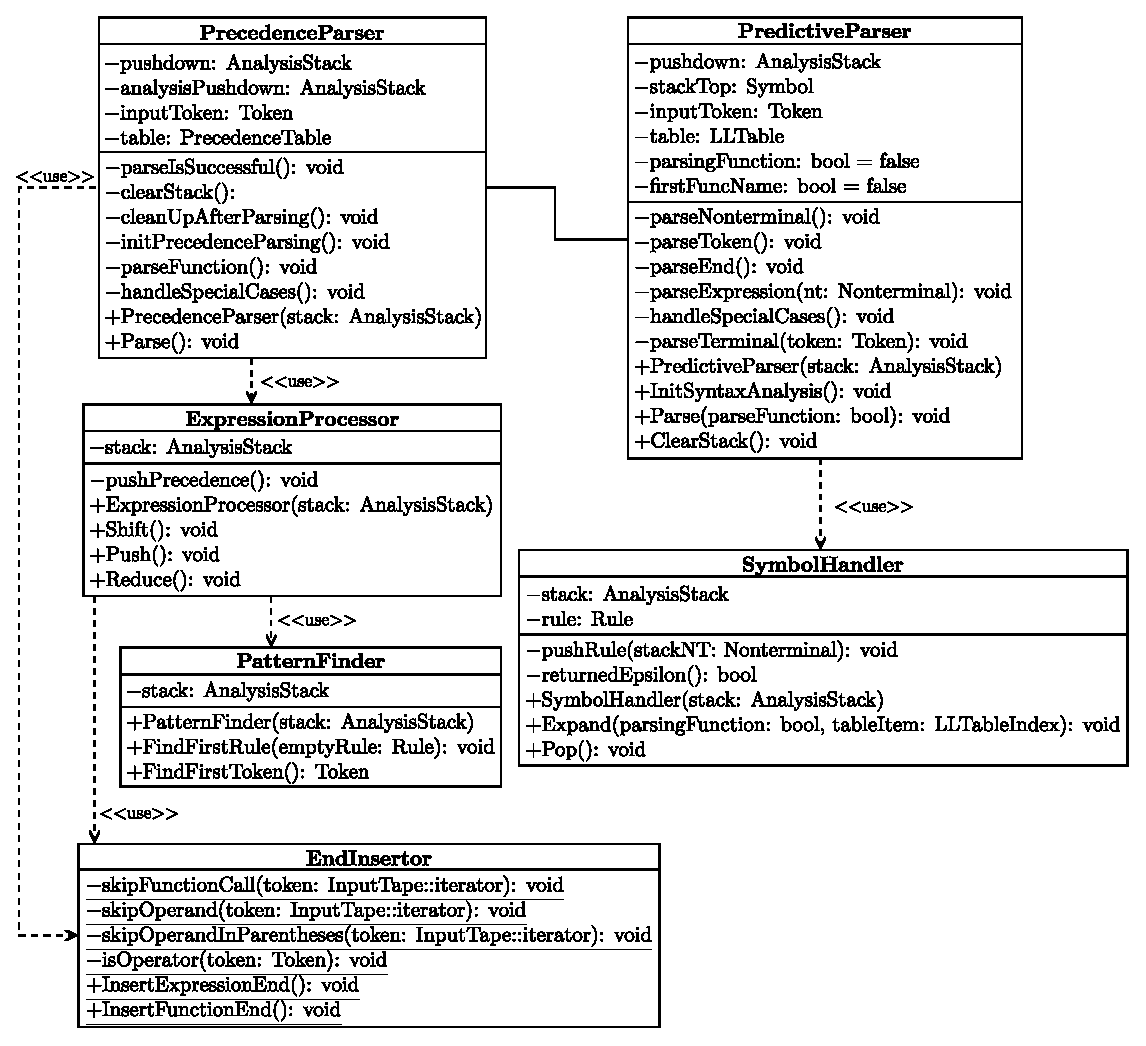
\includegraphics[width=0.92\textwidth]{obrazky-figures/parsers_class_diagram.eps}
    \caption{Vztahy mezi třídami, které spolupracují na syntaktické analýze.}
    \label{fig_parsers_class_diagram}
\end{figure}

\chapter{Třídní hierarchie uzlů AST} \label{kap_priloha_c}
Pro větší přehlednost je hierarchie rozdělena do tří obrázků.
Tyto diagramy jsou úmyslně zjednodušené, zaměřují se pouze na vzájemnou dědičnost mezi třídami; opomíjí kompoziční vztahy a~další detaily, jako například jiné a~ne tak podstatné třídy, použité enumerátory a~podobně.
Jejich hlavním účelem je ilustrovat strukturu hierarchie uzlů AST.

První obrázek (Obrázek \ref{fig_hierarchie_astnode}) ukazuje třídu \texttt{ASTNode} a~třídy, které z~ní přímo dědí.
\begin{figure}[h]
	\centering
	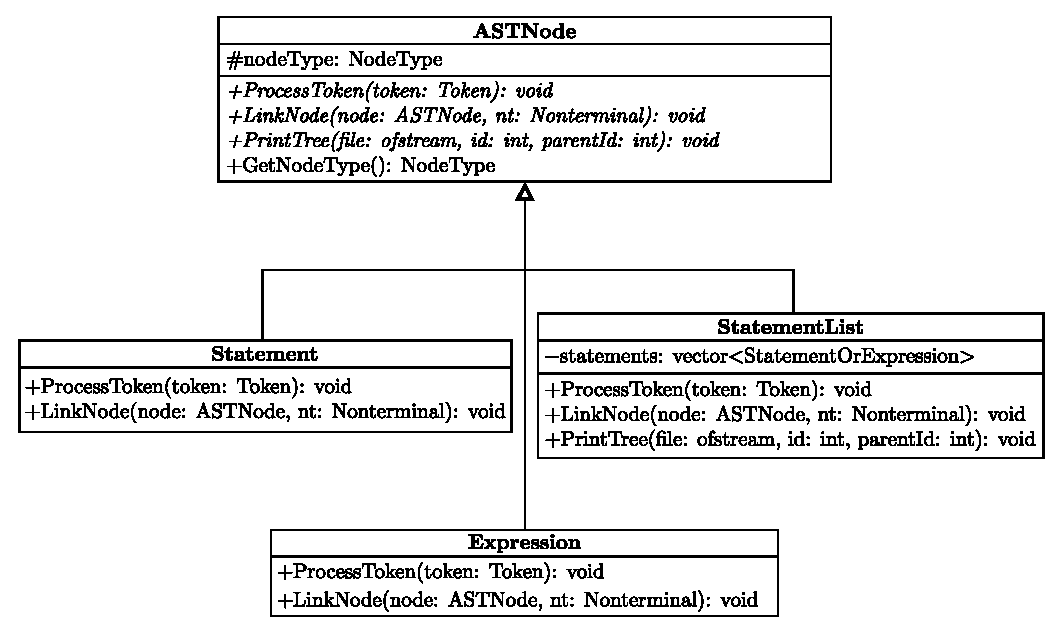
\includegraphics[width=\textwidth]{obrazky-figures/ast_node_hierarchy.eps}
	\caption{Diagram tříd zobrazující abstraktní třídu \texttt{ASTNode} a~její přímé potomky.}
	\label{fig_hierarchie_astnode}
\end{figure}
\newpage

Druhý obrázek (Obrázek \ref{fig_hierarchie_expression}) prezentuje hierarchii tříd, které reprezentují různé typy výrazů v~AST. 
\begin{figure}[h]
	\centering
	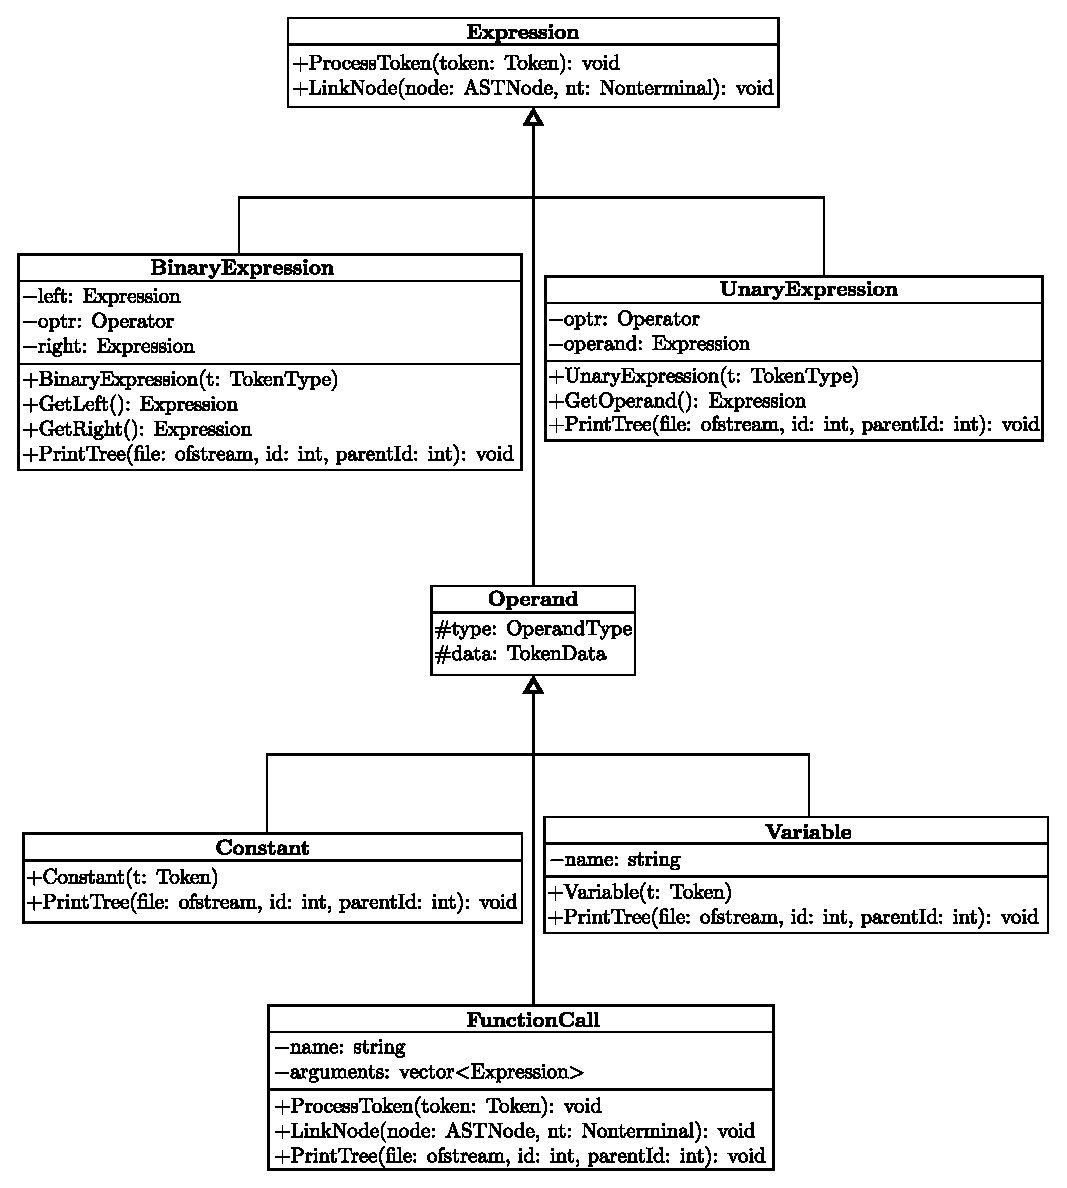
\includegraphics[width=\textwidth]{obrazky-figures/expression_hierarchy.eps}
\caption{Hierarchie tříd, které reprezentují výrazy v~AST.}
	\label{fig_hierarchie_expression}
\end{figure}
\newpage

Třetí diagram na Obrázku \ref{fig_hierarchie_statement} zobrazuje různé druhy příkazů ve zdrojovém kódu pomocí tříd.
Podobně jako u~předchozích diagramů, tento diagram se soustředí na hierarchii těchto tříd a~vynechává zbytečné detaily.
\begin{figure}[h!]
		\centering
		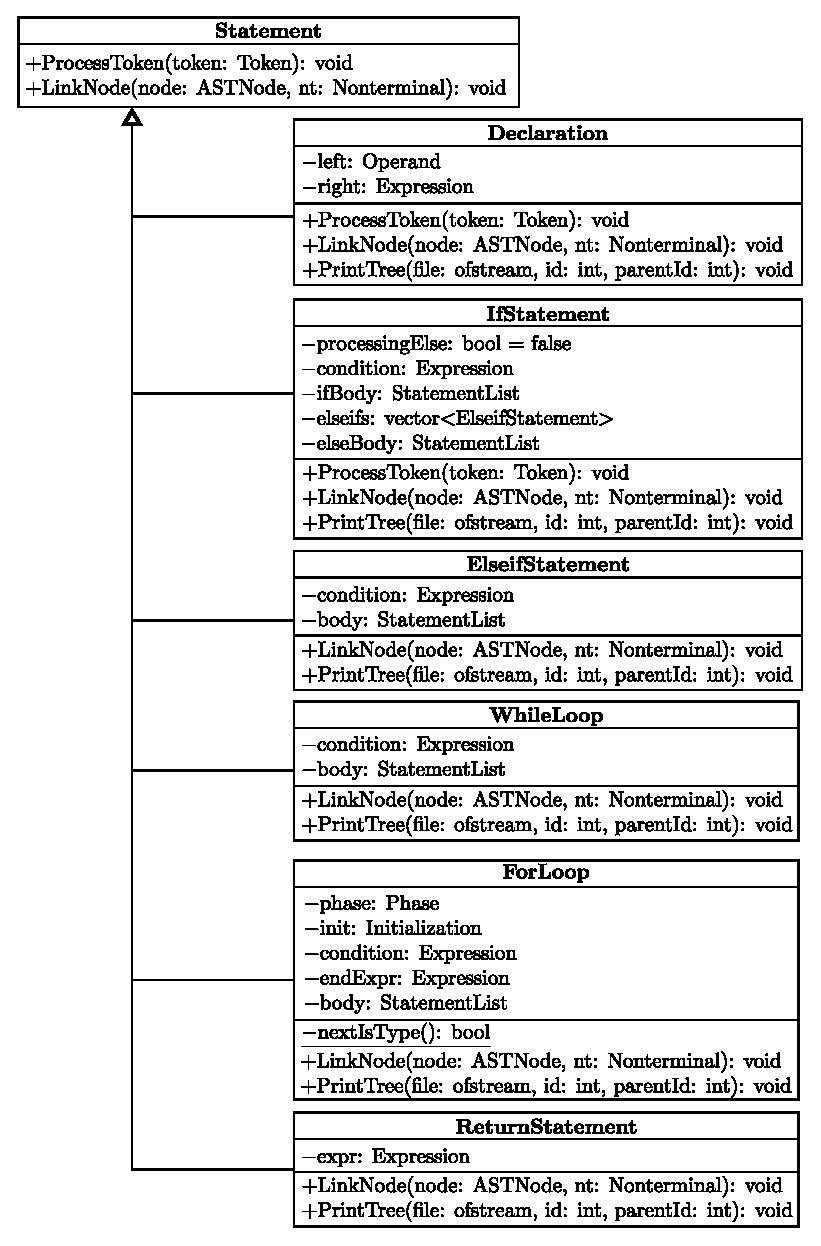
\includegraphics[height=0.88\textheight]{obrazky-figures/statement_hierarchy.eps}
		\caption{Hierarchie tříd, které reprezentují příkazy v~AST.}
		\label{fig_hierarchie_statement}
\end{figure}

\newpage

Poslední třída je \texttt{FunctionDefinition}.
Ta také dědí od třídy \texttt{Statement}, ale do předchozího diagramu nebyla zařazena ze dvou důvodů:
\begin{enumerate}
	\item sémanticky se do ostatních příkazů nehodí,
	\item diagram na Obrázku \ref{fig_hierarchie_statement} by byl takřka nečitelný kvůli velkému množství tříd, což by způsobilo oddálení diagramu.
\end{enumerate}
Proto je tato třída zobrazena v~samostatném diagramu na Obrázku \ref{fig_hierarchie_funcdef}.
K~této třídě byla přidána i~třída \texttt{Parameter}, která je nedílnou součástí definice funkce, a~agregační vztah mezi nimi.

\begin{figure}[h!]
	\centering
	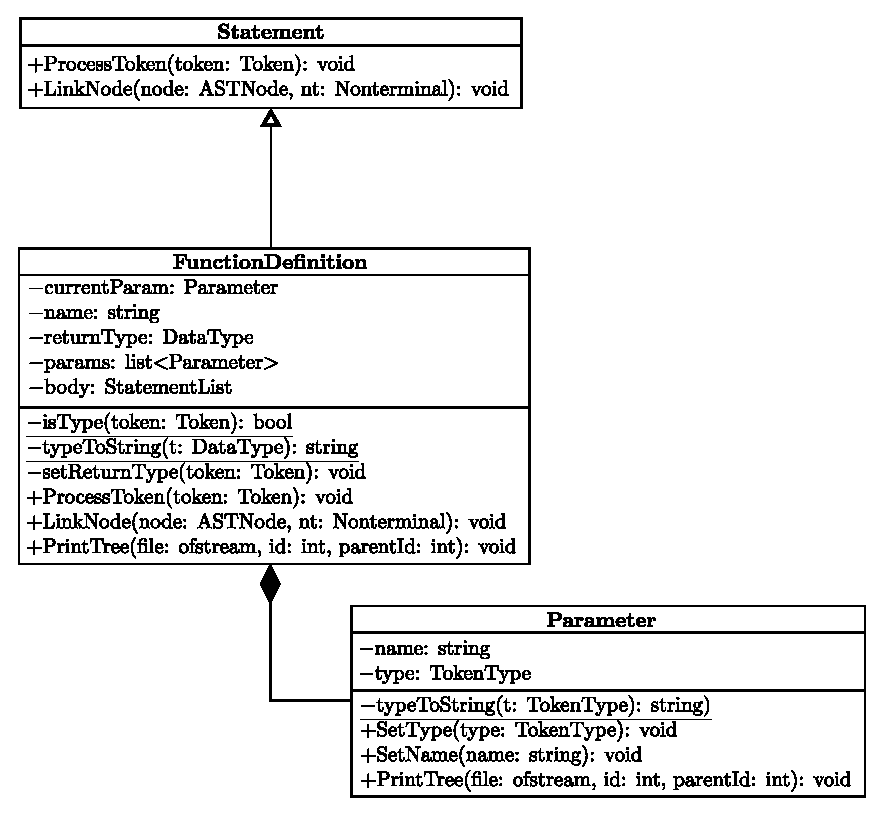
\includegraphics[width=\textwidth]{obrazky-figures/funcdef_hierarchy.eps}
	\caption{Diagram tříd zobrazující zařazení třídy \texttt{FunctionDefinition} do hierarchie uzlů AST.}
	\label{fig_hierarchie_funcdef}	
\end{figure}

\chapter{LL tabulka pro syntaktický analyzátor jazyka Koubp} \label{kap_priloha_d}

Protože celá LL tabulka je moc velká na to, aby se do přílohy vlezla celá, v~Tabulce \ref{tab_ll_table_priloha} je ukázka LL tabulky s~uspořádanými dvojicemi, kterou se tato práce zabývá a~která je jádrem implementovaného syntaktického analyzátoru pro jazyk Koubp.

\begin{table}[h]
	\centering
	\begin{tabularx}{\textwidth}{|l|c|c|c|c|c|c|c|c}
		\hline
		& \texttt{if} & \texttt{while} & \texttt{for} & \texttt{return} & \texttt{;} & \texttt{elseif} & \texttt{else} & $\cdots$ \\
		\hline
		\texttt{PROGRAM} & (1, 1) & (1, 1) & (1, 1) & (1, 1) & (1, 1) & (0, 0) & (0, 0) & $\cdots$\\
		\hline
		\texttt{STATEMENTLIST} & (1, 3) & (1, 3) & (1, 3) & (1, 3) & (1, 3) & (0, 0) & (0, 0) & $\cdots$\\
		\hline
		\texttt{STATEMENT} & (2, 1) & (2, 2) & (2, 3) & (2, 6) & (2, 7) & (0, 0) & (0, 0) & $\cdots$\\
		\hline
		\texttt{IF2} & (2, 10) & (2, 10) & (2, 10) & (2, 10) & (2, 10) & (2, 8) & (2, 9) & $\cdots$\\
		\hline
		\texttt{DECLOREXP} & (0, 0) & (0, 0) & (0, 0) & (0, 0) & (0, 0) & (0, 0) & (0, 0) & $\cdots$\\
		\hline
		\texttt{RETURNEXP} & (0, 0) & (0, 0) & (0, 0) & (0, 0) & (2, 14) & (0, 0) & (0, 0) & $\cdots$\\
		\hline
		\texttt{FUNCTIONDEF} & (0, 0) & (0, 0) & (0, 0) & (0, 0) & (0, 0) & (0, 0) & (0, 0) &$\cdots$ \\
		\hline
		\texttt{PARAMS} & (0, 0) & (0, 0) & (0, 0) & (0, 0) & (0, 0) & (0, 0) & (0, 0) & $\cdots$\\
		\hline
		\texttt{PARAMS2} & (0, 0) & (0, 0) & (0, 0) & (0, 0) & (0, 0) & (0, 0) & (0, 0) & $\cdots$\\
		\hline
		\texttt{EXPRESSION} & (0, 0) & (0, 0) & (0, 0) & (0, 0) & (0, 0) & (0, 0) & (0, 0) & $\cdots$ \\
		\hline
		\texttt{ARGS} & (0, 0) & (0, 0) & (0, 0) & (0, 0) & (0, 0) & (0, 0) & (0, 0) & $\cdots$ \\
		\hline
		\texttt{ARGS2} & (0, 0) & (0, 0) & (0, 0) & (0, 0) & (0, 0) & (0, 0) & (0, 0) & $\cdots$ \\
		\hline
		\texttt{CODEBLOCK} & (5, 2) & (5, 2) & (5, 2) & (5, 2) & (5, 2) & (0, 0) & (0, 0)& $\cdots$ \\
		\hline
		\texttt{STATEMENTS} & (5, 3) & (5, 3) & (5, 3) & (5, 3) & (5, 3) & (0, 0) & (0, 0) & $\cdots$ \\
		\hline
		\texttt{VOLTYPE} & (0, 0) & (0, 0) & (0, 0) & (0, 0) & (0, 0) & (0, 0) & (0, 0) & $\cdots$ \\
		\hline
		\texttt{TYPE} & (0, 0) & (0, 0) & (0, 0) & (0, 0) & (0, 0) & (0, 0) & (0, 0)& $\cdots$ \\
		\hline
	\end{tabularx}
	\caption{Část LL tabulky s~uspořádanými dvojicemi, která tvoří jádro syntaktického analyzátoru pro jazyk Koubp.}
	\label{tab_ll_table_priloha}
\end{table}


%\chapter{Plakát}



% Pro kompilaci po částech (viz projekt.tex) nutno odkomentovat
%\end{document}
